\documentclass[a4paper,12pt]{article} 
\usepackage{baseset}
\DeclareSymbolFont{operators}{OT1}{ntxtlf}{m}{n}
\SetSymbolFont{operators}{bold}{OT1}{ntxtlf}{b}{n}
\usepackage{wasysym}
\usepackage{multirow}
\graphicspath{{images/}}
\DeclareGraphicsExtensions{.pdf,.png,.jpg}

%Заговолок
\author{Красоткина Виктория}

\title{Лабораторная работа 1.2.1

Определение скорости полета пули при помощи баллистического маятника}

\date{7 ноября 2022 г.}

\begin{document}

\maketitle
\thispagestyle{empty}

\newpage
\setcounter{page}{1}

\textbf{Цель:}
Определить скорость полета пули, применяя законы сохранения и используя баллистические маятники.

\textbf{Приборы:}
\begin{itemize}
    \item духовое ружье на штативе
    \item осветитель
    \item оптическая система для измерения отклонений маятника
    \item измерительная линейка
    \item пули и весы для их взвешивания
    \item пинцет
    \item также баллистические маятники
\end{itemize}

\subsection*{Теоретическая часть}
Скорость вылета пули из духового ружья $150-200$ м/с, из боевой винтовки $1000$ м/с. Время пролета пули составляет величину порядка $10^{-2} -- 10^{-3}$ с. В данной работе будем определять скорость пули по импульсу, передаваемому ею некоторому телу при неупругом соударении. Импульс системы пуля -- тело сохраняется. Если масса тела значительно больше массы пули, то скорость тела с застрявшей в нем пулей будет значительно меньше скорости пули, и ее легче измерить. Длительность неупругого соударения пули и тела, измеряемая с моментах их соприкосновения до прекращения относительного движения, зависит от сопротивления, которое испытывает пуля при движении внутри тела. Оценить ее можно по глубине проникновения пули в тело, предполагая силу сопротивления постоянной.

Для измерения переданного пулей импульса используют баллистический маятник. Баллистическим называется маятник, колебания которого вызываются кратковременным начальным импульсом. Кратковременным можно считать импульс, если время действия сил (время соударения) значительно меньше периода колебаний маятника. При этом отклонение маятника за время соударения значительно меньше амплитуды колебаний. В случае гармонических колебаний время соударения $\tau$, отнесенное к периоду колебаний $T$, и отклонение $\Delta \varphi$ за время соударения, отнесенное к амплитуде, связаны соотношением 
$$
\frac{\Delta\varphi}{\varphi_{m}} \approx \frac{2\pi \tau}{T}
$$

Связь между максимальным отклонением маятника и начальной скоростью, полученной им в результате толчка, описывается законом сохранения механической энергии, если потери энергии за период значительно меньше энергии его колебаний. В дальнейшем будем считать затухание малым, если за $10$ колебаний амплитуда уменьшается меньше, чем наполовину. По начальному максимальному отклонению маятника определяются импульс и скорость пули.

После удара, пули колебания маятника должны происходить в одной плоскости.

Ружье закреплено на специальном штативе. Чтобы зарядить ружье, надо освободить стопорный винт штатива и наклонить ружье в держатель набок. Затем отогнуть ствол в сторону курка до упора, зарядить ружье и вернуть все в первоначальное состояние.
\begin{figure}[h]
    \centering
    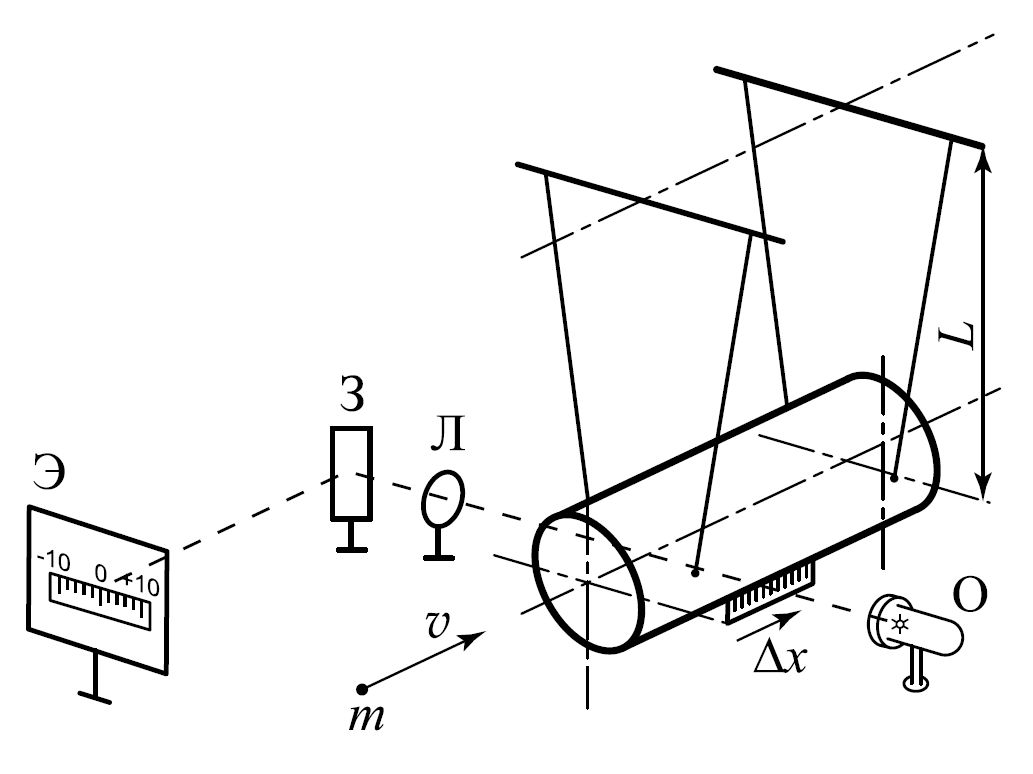
\includegraphics[width=0.7\textwidth]{1.2.1 1}
    \caption{Схема установки для измерения скорости полета пули}
    \label{1}
\end{figure}

\subsubsection*{Метод баллистического маятника, совершающего поступательное движение}

Используемый в этой части работы баллистический маятник представляет собой тяжелый цилиндр, подвешенный на четырех нитях одинаковой длины. Он изображен на рис. \ref{1} вместе с измерительной системой. Любая точка цилиндра при колебаниях маятника, движется по дуге окружности, радиус которой равен расстоянию по вертикали между уровнями верхнего и нижнего концов нитей подвеса. Это поясняется на рис. \ref{2} (вид сбоку, в плоскости колебаний). Все точки цилиндра движутся по дугам окружностей одинакового радиуса относительно соответствующих каждой точке центров, в частности, центр масс $M_0$ переходит в $M_1$ по дуге окружности с центром в точке $O$. Все радиусы одинаковы и обозначены $L$.

\begin{figure}[h]
    \centering
    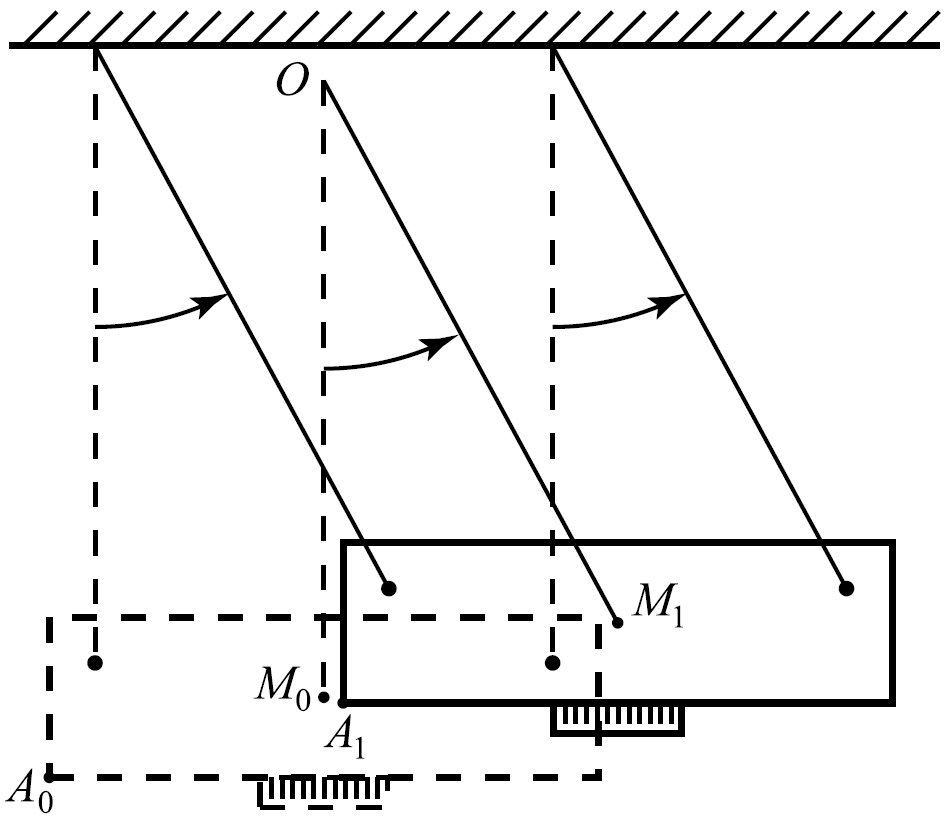
\includegraphics[width=0.7\textwidth]{1.2.1 2}
    \caption{Баллистический маятник, совершающий поступательное движение}
    \label{2}
\end{figure}

Закон сохранения импульса при соударении пули с цилиндром имеет вид 
$$
mu = (M + m)v
$$

Здесь $m$ -- это масса пули, $M$ -- масса цилиндра, $u$ -- скорость пули перед ударом, $v$ -- скорость цилиндра и пули после неупругого соударения.

Учитывая, что масса маятника значительно больше массы пули, можно написать
$$
u = \frac{M}{m}V
$$

Получив начальную кинетическую энергию, маятник при отклонении будет подниматься до тех пор, пока всю ее не израсходует. Если пренебречь потерями, то вся кинетическая энергия переходит в потенциальную в поле тяжести. Тогда по закону сохранения механической энергии высота $h$ подъема маятника над его начальным положением связана с начальной скоростью маятника $V$ следующим образом: 
$$
v^2 = 2gh
$$

Здесь $g$ -- ускорения свободного падения.

Высота подъема маятника выражается через угол $\varphi$ отклонения маятника от вертикали: 
$$
h = L(1 - \cos{\varphi}) = 2L \sin^2{\frac{\varphi}{2}},
$$
где $\varphi \approx \dfrac{\Delta x}{L}$.

Из всех вышеперечисленных получаем окончательную формулу для определения скорости пули:
\begin{equation}
\label{eq_vel}
u = \frac{M}{m}\sqrt{\frac{g}{L}}\Delta x
\end{equation}

Измерение отклонения маятника $\Delta x$ производится с помощью оптической системы, изображенной на рис. \ref{1}. По увеличенному изображению шкалы, закрепленной на цилиндре, определяется ее горизонтальное смещение. Таким образом может быть измерено максимальное отклонение маятника и изменение максимальных отклонений для определения затуханий колебаний.

Справедливость соотношения для $v^2 = 2gh$ и, следовательно, окончательной формулы обусловлена возможность пренебречь потерями энергии при колебаниях.

Среди причин, вызывающих затухание колебаний маятника, наиболее существенными являются трение о воздух и недостаточно жесткое закрепление точки подвеса.

\subsection*{Ход работы}
Сперва определим погрешности приборов:
\begin{itemize}
	\item линейка: $2\cdot\dfrac{\text{цена деления}}{2} = 1$ мм
	\item линейка на маятнике: из описания установки $0.25$ мм
	\item весы: из описания прибора $0.001$ г
\end{itemize}
Систематическую погрешность будем определять по формуле
$$
\sigma_{\text{сист}} = \sqrt{\frac{1}{N(N - 1)}\sum_{i = 1}^{N}(x_i - \langle x\rangle)^2}
$$
Общую погрешность найдем как среднеквадратичную величину из всех погрешностей:
$$
\sigma = \sqrt{\sigma^2_{\text{случ}} + \sigma^2_{\text{пр}} + \dots}
$$

\begin{enumerate}
    \item Ознакомимся с устройством баллистического маятника и измерительной установки, а так же научимся пользоваться духовным ружьем.
    \item Измерим на аналитических весах массу каждой пульки, полученной у лаборанта, поместим их в ячейки коробки под соответствующими номерами, чтобы не перепутать при использовании. Данные измерения привидены в таблице ниже:
    \begin{table}[h]
        \centering
        \begin{tabular}{|c|c|c|c|c|c|c|c|c|} \hline 
            $N$ & $1$ & $2$ & $3$ & $4$ & $5$ & $6$ & $7$ & $8$ \\ \hline
            $m$, г & $0.500$ & $0.512$ & $0.498$ & $0.503$ & $0.519$ & $0.507$ & $0.516$ & $0.513$ \\ \hline 
        \end{tabular} 
    \end{table}

    Первые четыре грузика будут учавствовать в первой части лабораторной работы, а другие четыре во второй соответственно.
    \item С помощью двухметровой метровой линейки измеряем расстояние $L$ (см. рис. \ref{1}). Полученные значения:
    \begin{table}[h]
        \centering
        \begin{tabular}{|c|c|c|c|c|c|} \hline 
            $N$ & $1$ & $2$ & $3$ & $4$ \\ \hline
            $L$, см  & $222$ & $221$ & $222$ & $222$ \\ \hline 
        \end{tabular}
    \end{table}
    
    Среднее значение: 
    $$
    \langle L\rangle = \frac{1}{N}\sum_{i = 1}^{N} L_i = 221.8~\text{см}
    $$
    Приборная погрешность -- $0.1$ см.

    Систематическая погрешность -- $0.25$ см.

    Итоговый ответ:
    $$
    \langle L\rangle = 221.8 \pm 0.3~\text{см}
    $$
    Так же $M = 2900 \pm 5$ г.

    \item Собираем оптическую систему, предназначенную для измерения перемещения маятника. Включаем осветитель и добиваемся четкого изображения шкалы на экране.
    \item После произведения холостого выстрела по маятнику убедились, что влияние полностью отсутствует.
    \item Возбудим колебания. Амплитуда вначале была равна $12.5$ мм. После $10$ колебаний амплитуда стала равна $12.0$ мм, то есть уменшилась на $4\%$ -- отсюда вывод, что затухание колебаний мало.
    \item Проводим выстрелы пуль из ружья, при этом замеряя отклонения $\Delta x$. Построим таблицу полученных данных:
    \begin{table}[h]
        \centering
        \begin{tabular}{|c|c|c|c|c|} \hline 
            $N$ & $5$ & $6$ & $7$ & $8$ \\ \hline 
            $m$, г & $0.519$ & $0.507$ & $0.516$ & $0.513$ \\ \hline 
            $\Delta x$, мм & $13$ & $12.25$ & $12.25$ & $12.5$ \\ \hline 
            $u$, м/с & $142.4$ & $145.0$ & $141.1$ & $143.3$ \\ \hline
            $\sigma_u$, м/с & $3.0$ & $3.0$ & $3.0$ & $3.0$ \\ \hline
            $u_0$, м/с & $148.6$ & $144.8$ & $147.4$ & $152.8$ \\ \hline
            \end{tabular}
        \caption{Измерения для первой установки}
        \label{table1}
    \end{table}

    Для каждого измерения рассчитаем скорость пули при выстреле по формуле \ref{eq_vel}. Значения запишем в таблицу \ref{table1}. Кроме того, мы измеряли скорость при помощи спидометра, расположенного напротив дула ружья: запишем значения $u_0$ в таблицу \ref{table1}.

    \item Оценим погрешность определения скорости пули в каждом выстреле. Вклад вносит только приборная погрешность:
    \begin{multline*}
        \sigma_{u} = \sqrt{\left(\frac{\partial{u}}{\partial{M}}\right)^2\cdot\sigma_M^2 + \left(\frac{\partial{u}}{\partial{L}}\right)^2\cdot \sigma_L^2 + \left(\frac{\partial{u}}{\partial{\Delta x}}\right)^2\cdot \sigma_{\Delta x}^2 + \left(\frac{\partial{u}}{\partial{m}}\right)^2\cdot \sigma_{m}^2} = \\
        = \sqrt{\frac{g\Delta x^2}{m^2L}\cdot \sigma_M^2 + \frac{M^2g\Delta x^2}{4m^2L^3}\cdot \sigma_L^2 + \frac{M^2g}{m^2L}\cdot \sigma_x^2 + \frac{M^2\Delta x^2g}{L^2 m^4}\cdot \sigma_m^2}
    \end{multline*}
    Погрешности каждого измерения запишем в таблицу \ref{table1}.
    
    \item Рассчитаем среднее значение скорости пули:
    $$
    \langle u\rangle = \frac{1}{N}\sum_{i = 1}^{N} u_i = 143.0~\text{м/с}
    $$
    Погрешности величины скорости:
    $$
    \sigma_u^{\text{случ}} = 0.8~\text{м/с},~\sigma_u^{\text{пр}} = 0.3~\text{м/с},~\sigma_u = 3.1~\text{м/с}
    $$
    Итоговый ответ: 
    $$
    u = 143.0 \pm 3.1~\text{м/с}
    $$
    В нашем случае больший вклад в ошибку вносит приборная погрешность. 
\end{enumerate}
\subsection*{Вывод}
Мы определили скорость полета пули и погрешность этой величины, используя баллистический маятник, совершающий поступательное движение. Мы получили значение, согласующееся с теоретическими данными ($143.0$ м/с), с приемлемой точностью. Основной вклад в ошибку найденной величины вносит приборная погрешность.

\newpage

\subsubsection*{Метод крутильного баллистического маятника}

Схема эксперимента изображена на рис. \ref{3}. Пуля массой $m$ попадает в мишень, укрепленную на стержне $aa$, который вместе с грузами $M$ и проволокой П образует крутильный маятник. Считая удар пули о мишень неупругим, для определения скорости $u$ полета пули непосредственно перед ударом воспользуемся законом сохранения момента импульса в виде 
\begin{equation}
    \label{eq_I}
    mur = I\Omega
\end{equation}
На рисунке \ref{3}: $r$ -- расстояние от линии полета пули до оси вращения маятника (до проволоки П), $I$ -- момент инерции маятника, $\Omega$ -- его угловая скорость непосредственно после удара.

\begin{figure}[h]
    \centering
    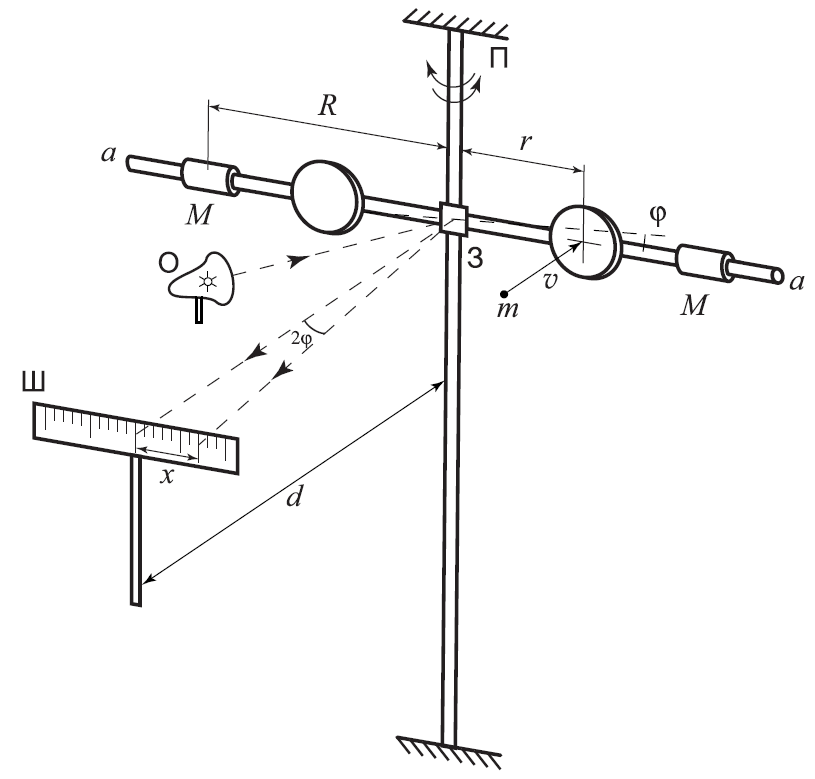
\includegraphics[width=0.7\textwidth]{1.2.1 3}
    \caption{Крутильный баллистический маятник}
    \label{3}
\end{figure}

Законом созранения момента импульса можно воспользоваться, если время соударения пули с мишенью значительно меньше периода малых колебаний маятника.

Начальная кинетическая энергия вращения маятника переходит в потенциальную -- упругую энергию закручивания проволоки и расходуется на необратимые потери -- в первую очередь на трение о воздух. Роль потерь можно оценить по изменению амплитуды колебаний за $10$ периодов. Если амплитуда уменьшается менее чем наполовину, то затухание колебаний считаем малым, то есть потери энергии за период колебаний значительно меньше энергии колебаний. Пренебрегая потерями, закон сохранения энергии при колебаниях записываем следующим образом: 
\begin{equation}
    \label{eq_k}
    k\frac{\varphi^2}{2} = I\frac{\Omega^2}{2},
\end{equation}
где $k$ -- модуль кручения проволоки П, а $\varphi$ -- максимальный угол поворота маятника.

Из (\ref{eq_I}) и (\ref{eq_k}) получаем 
\begin{equation}
    \label{eq_u}
    u = \varphi\frac{\sqrt{kI}}{mr}
\end{equation}

Угол максимального закручивания маятника в данных опытах всегда мал и легко находится по смещению $x$ изображения нити осветителя на измерительной шкале. Из рис. \ref{3} следует
\begin{equation}
    \label{eq_varphi}
    \varphi \approx \frac{x}{2d},
\end{equation}
где $d$ -- расстояние от шкалы Ш до оси вращения маятника.

В формулу (\ref{eq_u}) входит произведение $kI$, которое можно найти по измерениям периодов колебаний маятника с грузами $M$ и без них. В первом случае период колебаний равен: 
\begin{equation}
    \label{eq_t1}
    T_1 = 2\pi \sqrt{\frac{I}{k}}
\end{equation}
Во втором случае 
\begin{equation}
    \label{eq_t2}
    T_2 = 2\pi \sqrt{\frac{I - 2MR^2}{k}}
\end{equation}

Из (\ref{eq_t1}) и (\ref{eq_t2}) следует 
\begin{equation}
    \label{eq_kI}
    \sqrt{kI} = \frac{4\pi MR^2T_1}{T_1^2 - T_2^2},
\end{equation}
где $R$ -- расстояние от центров масс грузов $M$ до проволоки.

\subsection*{Ход работы}
\begin{enumerate}
    \item Изучим и ознакомимся с конструкцией установки, а так же научимся пользоваться духовым ружьем.
    \item Массы пулек уже были измерены в первой части опыта.
    \item Измерим парметры установки:
    $$
    r = 23.0 \pm 0.1~\text{см},~R = 35.0 \pm 0.1~\text{см},~d = 46.0 \pm 0.1~\text{см}
    $$
    Массы грузов: $M_1 = 713.9 \pm 0.1$ г, $M_2 = 714.1 \pm 0.1$ г. Тогда
    $$
    M = \frac{M_1 + M_2}{2} = 714.0 \pm 0.1~\text{г}
    $$

    \item Настраиваем оптическую система, предназначенную для измерения поворота маятника. Включаем осветитель О, направляем свет на зеркальце З и получаем четкое изображение нити осветителя на шкале.
    \item Холостой выстрел уже был произведен в начале работы, и мы убедились, что маятник практически не реагирует на воздушную струю из ружья.
    \item Возбудим колебания. Амплитуда вначале была равна $13.6$ мм. После $10$ колебаний амплитуда стала равна $12.9$ мм, то есть уменшилась на $5\%$ -- отсюда вывод, что затухание колебаний мало.
    \item Измеряем время $10-15$ полных крутильных колебаний маятника, при помощи секундомера, определяем $T_1$ и $T_2$. Измеряем периоды несколько раз, чтобы получить более точные данные. Таблица полученных данных:
    \begin{table}[h]
        \centering
        \begin{tabular}{|c|c|c|c|c|} \hline 
            $N$ & $1$ & $2$ & $3$ & $4$ \\ \hline 
            $10T_1$, c& $179.50$ & $179.20$ & $180.1$ & $178.8$ \\ \hline 
            $10T_2$, c& $135.80$ & $134.60$ & $135.90$ & $135.7$ \\ \hline 
            $T_1$, c& $17.95$ & $17.92$ & $18.01$ & $17.88$ \\ \hline 
            $T_2$, c& $13.58$ & $13.46$ & $13.59$ & $13.57$ \\ \hline 
        \end{tabular} 
    \end{table}
    
    Средние значения периодов:
    $$
    \langle T_1 \rangle = 17.94~\text{с},~\langle T_2 \rangle = 13.55~\text{с}
    $$
    Так как периоды $T$ измерялись с помощью телефонного секундомера, то $\sigma^{\text{пр}}_T = 0.01$ c. 
    
    Случайные погрешности:
    $$
    \sigma^{\text{случ}}_{T_1} = 0.03~\text{с},~\sigma^{\text{случ}}_{T_2} = 0.03~\text{с}
    $$ 
    Итоговые величины периодов:
    $$
    T_1 = 17.94 \pm 0.03~\text{с},~ T_2 = 13.55 \pm 0.03~\text{с}
    $$
    По формуле (\ref{eq_kI}) найдем величину $\sqrt{kI}$ и оценим ее погрешность.
    $$
    \sqrt{kI} = \frac{4\pi MR^2T_1}{T_1^2 - T_2^2} = 0.144~\frac{\text{кг}\cdot\text{м}^2}{\text{с}}
    $$
    Погрешность рассчитывается по формуле
    \begin{multline*}
        \sigma_{\sqrt{kI}} = \sqrt{\left(\frac{\partial{\sqrt{kI}}}{\partial{M}}\right)^2\cdot\sigma_M^2 + \left(\frac{\partial{\sqrt{kI}}}{\partial{R}}\right)^2\cdot \sigma_R^2 + \left(\frac{\partial{\sqrt{kI}}}{\partial{T_1}}\right)^2\cdot \sigma_{T_1}^2 + \left(\frac{\partial{\sqrt{kI}}}{\partial{T_2}}\right)^2\cdot \sigma_{T_2}^2} = \\
        = \sqrt{\left(\frac{4\pi R^2 T_1}{T_1^2 - T_2^2}\right)^2 \cdot \sigma_M^2 + \left(\frac{8\pi MRT_1}{T_1^2 - T_2^2}\right)^2\cdot \sigma_R^2 + \left(\frac{4\pi MR^2\left(T_1^2 + T_2^2\right)}{\left(T_1^2-T_2^2\right)^2}\right)^2\cdot \sigma_{T_1}^2 +} \\ 
        \overline{+ \left(\frac{8\pi MR^2T_1T_2}{\left(T_1^2-T_2^2\right)^2}\right)^2\cdot \sigma_{T_2}^2} = 0.002~\frac{\text{кг}\cdot\text{м}^2}{\text{с}}
    \end{multline*}
    Итоговый ответ:
    $$
    \sqrt{kI} = (1.44 \pm 0.02) \cdot 10^{-1}~\frac{\text{кг}\cdot\text{м}^2}{\text{с}}
    $$

    \item Произведем несколько выстрелов, замеряя $x$, и по формулам (\ref{eq_u}) и (\ref{eq_varphi}) определим скорость пули при каждом выстреле. Таблица полученных данных: 
    \begin{table}[h]
        \centering
        \begin{tabular}{|c|c|c|c|c|}
            \hline 
            $N$ & $1$ & $2$ & $3$ & $4$ \\ \hline 
            $m$, г & $0.500$ & $0.512$ & $0.498$ & $0.503$ \\ \hline 
            $x$, см & $11.1$ & $11.7$ & $11.2$ & $11.5$ \\ \hline
            $\varphi$, рад & $0.121$ & $0.127$ & $0.122$ & $0.125$ \\ \hline
            $u$, м/с & $151.1$ & $155.5$ & $153.0$ & $155.6$ \\ \hline
        \end{tabular} 
    \end{table}
    Среднее значение скорости:
    $$
    \langle u \rangle = 153.8~\text{м/с}
    $$

    \item Оцениваем погрешность определения скорости пули в каждом выстреле по полученным данным.
    $$
    u = \varphi \frac{\sqrt{kI}}{mr}
    $$
    Приборная погрешность определения скорости:
    \begin{multline*}
        \sigma^{\text{пр}}_u = \sqrt{\left(\frac{\partial{u}}{\partial{\varphi}}\right)^2\cdot\sigma_M^2 + \left(\frac{\partial{u}}{\partial{\sqrt{kI}}}\right)^2\cdot \sigma_R^2 + \left(\frac{\partial{u}}{\partial{m}}\right)^2\cdot \sigma_{m}^2 + \left(\frac{\partial{u}}{\partial{r}}\right)^2\cdot \sigma_{r}^2} = \\
        = \sqrt{\left(\frac{\sqrt{kI}}{mr}\right)^2\cdot\sigma^2_{\varphi} + \left(\frac{\varphi}{mr}\right)\cdot\sigma^2_{\sqrt{kI}} + \left(\frac{\varphi\sqrt{kI}}{rm^2}\right)^2\sigma^2_m + \left(\frac{\varphi\sqrt{kI}}{r^2m}\right)\sigma^2_r} = 2.6~\text{м/с}
    \end{multline*}
    При этом
    $$
    \sigma_{\varphi} = \sqrt{\left(\frac{1}{2d}\right)^2\cdot \sigma_x^2 + \left(\frac{x}{2d^2}\right)^2\cdot \sigma_d^2 } = 0.001~\text{рад}
    $$
    Случайная погрешность: $\sigma_{\varphi}^{\text{случ}} = 1.1~\text{м/с}$
    Итого:
    $$
    u = 153.8 \pm 2.8~\text{м/с}
    $$
\end{enumerate}
\subsection*{Вывод}

Полученные значения скорости пули в разных частях не совсем совпадают в пределах погрешности. Полученный разброс связан в основном с разной скоростью от выстрела к выстрелу ружья (так как разные части лабораторной работы производились при помощь разных ружьев, а скорость выстрела на прямую зависит от накаченности баллона).Так же она сильно варьируется из-за разных форм пуль и других различных факторов. Так же можно сказать, что результат частично связан с погрешностью измерений и используемых приближений при проведении работы.
\end{document}


